We now look at more challenging scenarios where we show that the 
default MPTCP architecture is unable to adapt, resulting in sub-optimal 
performance which is often worse than that of SPTCP over the
faster subflow.

\begin{figure*}[h]
    \centering
    \subfigure[Network scan: Throughput timeline] {
        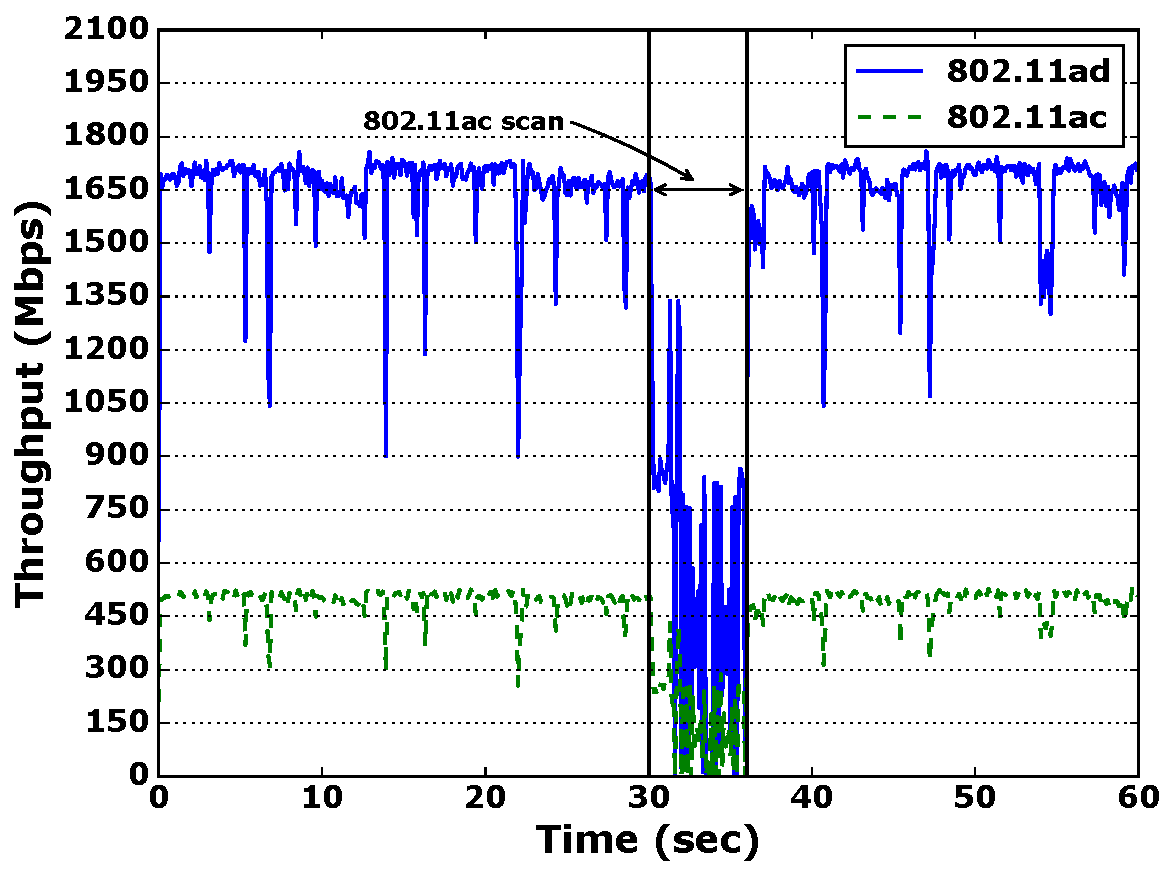
\includegraphics[scale=0.27]{NetworkManagerScan/timeline_no_fix.pdf}
        \label{fig:scan_issue}
    }\hfill
    \subfigure[802.11ac contention: Timeline showing throughput drop during contention] {
        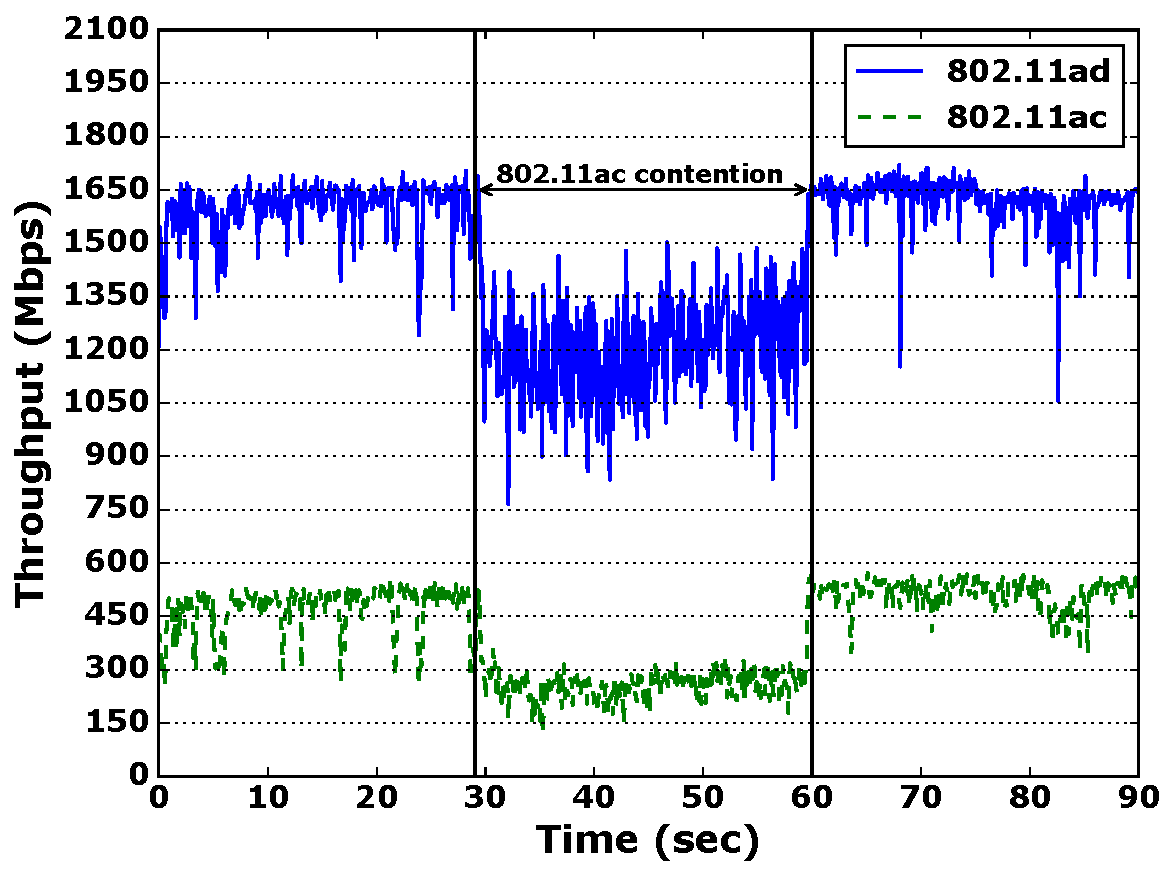
\includegraphics[scale=0.27]{contention/timeline.pdf}
        \label{fig:contention_timeline}
    }\hfill
    \subfigure[802.11ad blockage: 802.11ad throughput drop after re-connection] {
        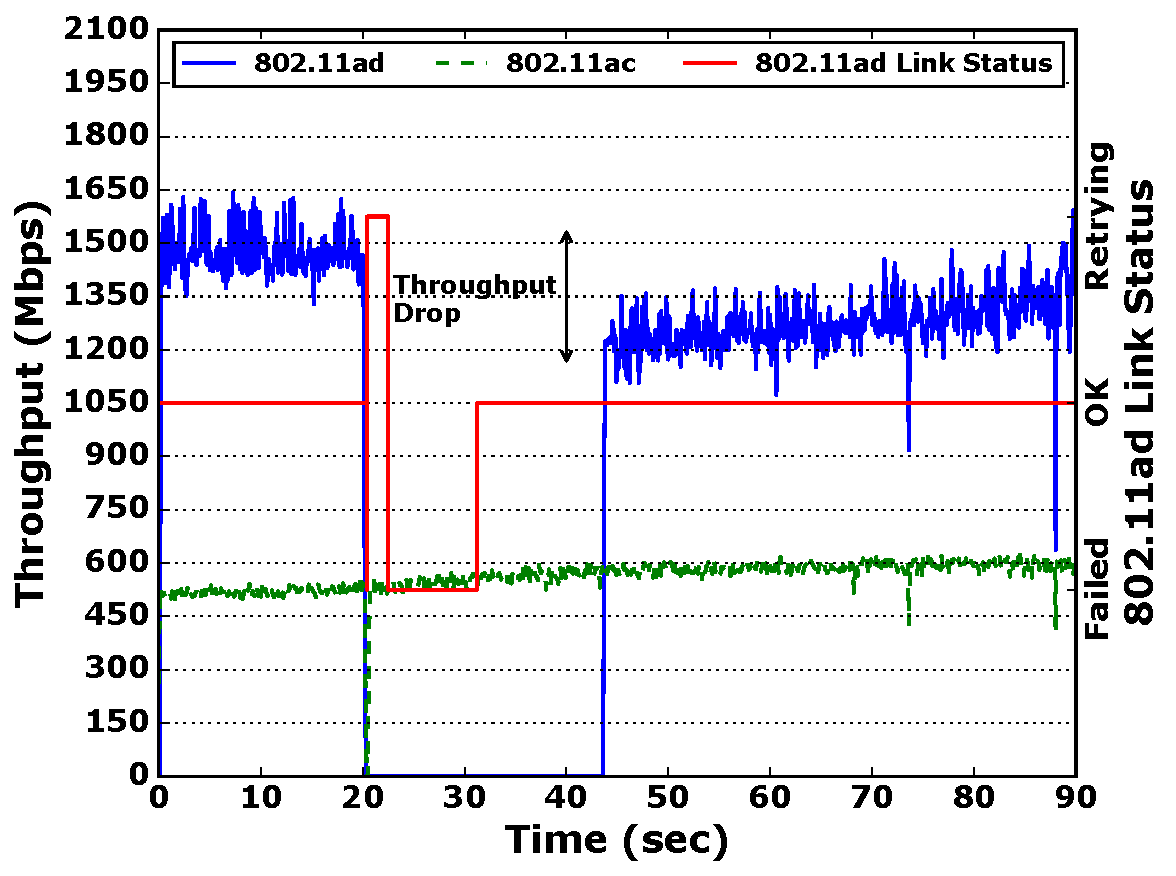
\includegraphics[scale=0.27]{blockage/blockage_tput_drop.pdf}
        \label{fig:blockage_tput_drop}
    }
    \vspace{-0.15in}
    \caption{Performance issues}
    \vspace{-0.1in}
\end{figure*}

\noindent\textbf{Network Scans. }Fig.~\ref{fig:scan_issue} shows the throughput of 802.11ad
and 802.11ac subflows over 60 s and the scan initiated at the 30 s mark. The 802.11ac throughput 
is cut down severely during the scan period (marked as "802.11ac scan") that lasts for 
around 6 s. This is an expected effect of the network scan as the radio is unable to
transmit regular data frames during this period. However, we observe that the 802.11ad 
flow is also impacted negatively during this period, even though the scan takes place in the 
5 GHz band. On investigation, we observed a 6x increase in the amount of data held in 
the \emph{ofo-queue} at the receiver end. During the scan period, the packet
scheduler, which is not aware of the sudden reduction in 802.11ac channel capacity, assigns 
packets in the same ratio as before the scan. This is problematic as the receiver's packet stream now has
\textit{gaps} (missing in-sequence packets) due to stuck 802.11ac packets; these gaps are 
preventing the receiver from delivering packets to the application until the missing packets arrive
or are re-transmitted over the 802.11ad interface.

\noindent\textbf{WiFi (802.11ac) Contention. } Fig.~\ref{fig:contention_timeline} shows a timeline of the
per-flow throughput of a 180 s MPTCP session. We start with a static link where 802.11ad and 802.11ac are 
at their maximum throughputs of $\sim$550 Mbps and $\sim$1650 Mbps, respectively, and we introduce
contention with 300 Mbps TCP cross-traffic at the 30th second for 30 s. The throughput of the 
802.11ac subflow drops by 300 Mbps to around 250 Mbps, as expected. Surprisingly, the 802.11ad subflow is also
affected negatively during the contention period with its throughput dropping below 1200 Mbps and experiencing more variability
than in the interval preceding the start of the contention period. In fact, the MPTCP throughput during the 
contention period averages to $\sim$1450(=1200+250) Mbps, which is less than even that of 802.11ad
operating alone (1650 Mbps). Note that 802.11ad channel capacity is unchanged as the contention is introduced 
only on the 802.11ac's operating channel. On further investigation, we found that during the
contention period the receiver advertised buffer space (\emph{recv\_win}) reduces significantly. 
Remember that the \emph{recv\_win} is maintained at the meta-level and, although
advertised on both subflows, is actually shared among them. Under such a scenario, the meta-level global sequence numbers
cannot advance, even though \emph{cwnd} allows for it, since the
meta-level buffers at the receiver are full, resulting in reduction of
throughput on both interfaces.

\noindent\textbf{60 GHz (802.11ad) Blockage. } Fig. \ref{fig:blockage_tput_drop} shows a
timeline of subflow throughputs along with link status {\tt Failed/OK/Retrying} as reported by 
the 802.11ad driver. The blockage is introduced at the $20^{th}$ second causing the link status 
to switch to fail after a further 2 s. Once the blockage is removed, connection at the MAC layer is
restored at the $30^{th}$ second. We observe the following two issues:
\\
(i) Although the 802.11ad link is restored at the $30^{th}$ second, MPTCP does not resume traffic 
on the 802.11ad subflow for another $\sim$20 seconds until the $49^{th}$ second. We found that
In the case of a timeout-based loss event, TCP congestion-control sets the {\tt pf} flag on the socket,
indicating the flow to be \emph{potentially failed}. The MPTCP scheduler treats subflows with 
the {\tt pf} flag set as being unavailable and does not schedule any packets on them. TCP
congestion-control, on the other hand, is waiting for an ACK to unset
the {\tt pf} flag and enter the {\tt TCP\_CA\_RECOVERY} state that can
restore the \emph{cwnd} to the value before the loss event. Since no
packets are being directed to the 802.11ad subflow, only a subflow-level re-transmission 
of the 802.11ad subflow can trigger the transmission of an ACK on the receiver side. However, 
multiple timeout-based losses during the blockage period can lead to excessively 
high retransmission timeouts, and consequently to long delays before an ACK is received after 
reconnection.
\\
(ii) On resumption, 802.11ad flow starts with a \emph{cwnd} and
\emph{ssthresh} that are half of their pre-loss values. Fig. \ref{fig:blockage_tput_drop} shows 
a sample timeline where the 802.11ad flow resumes to 1350 Mbps instead of 1650 Mbps. Note that
this behavior depends on the exact specifics of the TCP congestion-control state at the time 
it enters the recovery state. Nonetheless, we observed this quite often and it does have a
non-negligible impact on throughput.
